\chapter{The Lorentz and Poincar\'e Groups}\label{lorentz}

Now that we have identified the representations of the Euclidean group, we have established firm connections between most tangible physical actions and ways to analyze them through linear algebra techniques. Raising dimensions leaves us with a very limited understanding of the physical bearing of what our representations will truly embody. However, not all hope is lost in this regard. In this chapter, we introduce the Lorentz and Poincar\'e Groups, which are generalizations of four-dimensional space designed to embody properties of modern physics. In these spaces, our calculations will differ from those in prototypical four-dimensional space due to a relativistic paradigm shift. Our time component (which is the fourth dimension) will add negative weight to each vector's norm, leading to many failures of the normed linear structure that we are inherently used to. In more explicit terms, our space will obey the Minkowski metric as opposed to our standard Euclidean metric, which we will discuss in more detail below. This development will lead to a unique decomposition of our space and some physically meaningful interpretations. This chapter follows the structure laid out in Wu-ki Tung's \textit{Group Theory in Physics}. \cite{Tung}


\section{Construction and Basic Properties}

\begin{definition}
	An \textbf{event} is an ordered triple together with an additional parameter, meant to represent time. An event is conventionally indexed by the integers $\mu = 0,1,2,3$. Referring to an event as $x$ references the event a four (component) vector, and specifying $x^{\mu=0}$ gives us $ct$ where $c$ is the speed of light and $t$ is a time. 
\end{definition}

Our natural inclination is to believe that these vectors are just elements of $\R^4$. However, since this system is based on physical phenomena, the setup is a little more complicated.

\begin{definition}
	The \textbf{length} of an event is defined by the following equation:
$$\mid x\mid^2 \coloneq (x^1)^2+(x^2)^2+(x^3)^2 - (x^0)^2 = (x^1)^2+(x^2)^2+(x^3)^2 - c^2t^2$$
\end{definition}

We can immediately see that this four-dimensional length functional does not define a norm on this vector space, seeing as it is not positive-definite. This is in contrast to our conventional Euclidean norm. We cast both functionals into the context of matrix multiplication:

$$\begin{array}{c@{\hskip 1cm}c}

	\underset{\text{Euclidean Norm}}{||x||^2} = x^\intercal\begin{bmatrix}
													1 & 0 & 0 & 0\\
													 0 & 1 & 0 & 0\\
													0 & 0 & 1 & 0\\
													0 & 0 & 0 & 1
												\end{bmatrix}x

&
	\underset{\text{Length}}{|x|^2} = x^\intercal\begin{bmatrix}
													-1 & 0 & 0 & 0\\
													 0 & 1 & 0 & 0\\
													0 & 0 & 1 & 0\\
													0 & 0 & 0 & 1
												\end{bmatrix}x

\end{array}$$

In this light, entries along the diagonal of the $4\times 4$ matrix are what determine the value of the functional. Each of these matrices is referred to as a metric on this space, and it is clear that our space will inheret new structure as a consequence of the (latter) Minkowski metric.

\begin{definition}
	The \textbf{signature} of the length functional is the ordered quadruple of its diagonal elements $(-1,1,1,1)$.
\end{definition}

Before, we thought of our rotations and translations as being length-preserving operations. But in this four-dimensional space, what we define as length changes to be a less intrinsic measurement. As a result, discussing transformations that ``preserve length" will grow in complexity. A transformation can increase spatial components while decreasing a time component, leaving our length measure unaltered. This will have physical implications to be discussed later. For now, we will introduce our first group of interest

\begin{definition}
	A \textbf{Homogeneous Lorentz Transformation} is a continuous, length-preserving, linear transformation defined on our space-time vector space. By convention, we refer to such maps with the variable $\Lambda$.
\end{definition}

Naturally, we are taking the new meaning for the word length. Given that such transformations are linear, we can always represent this mapping as a matrix product (by some fixed matrix $\Lambda$). Explicitly, if we take $x = \sum_{\mu=0}^3 x^\mu e^\mu$ where $\{e^\mu\}$ is the standard basis and $x'$ to be the image under a homogeneous Lorentz transformation $\Lambda$, then

\begin{equation}
\begin{aligned}
	x' &= \Lambda x \\
		&= \sum_{\mu=0}^3 x^\mu \Lambda e^\mu \\
		&=  \sum_{\mu=0}^3 x^\mu \sum_{\nu=0}^3 [\Lambda]_{\nu\mu} e_\nu \\
		&= \sum_{\nu=0}^3 \left(\sum_{\mu=0}^3 x^\mu [\Lambda]_{\nu\mu} \right) e_\nu 
\end{aligned}
\end{equation}

with the restriction in place that 
\begin{small}
\begin{equation}
\begin{aligned}
	|x'|^2 &= |x|^2 \\ &\Leftrightarrow \\ \left(\sum_{\mu=0}^3 x^1[\Lambda]_{1\mu}\right)^2 +  \left(\sum_{\mu=0}^3 x^2[\Lambda]_{2\mu}\right)^2 +  \left(\sum_{\mu=0}^3 x^3[\Lambda]_{3\mu}\right)^2 - \left(\sum_{\mu=0}^3 x^0[\Lambda]_{0\mu}\right)^2 &= (x^1)^2 + (x^2)^2 + (x^3)^2 - (x^0)^2
\end{aligned}
\end{equation}
\end{small}

We can view this restriction in the context of the signature of the length by using the following:

\begin{equation}
\begin{aligned}
	\begin{bmatrix}
		x^0\sum_{\mu=0}^3 [\Lambda]_{0\mu}&
		x^1\sum_{\mu=0}^3 [\Lambda]_{1\mu}&
		x^2\sum_{\mu=0}^3 [\Lambda]_{2\mu}&
		x^3\sum_{\mu=0}^3 [\Lambda]_{3\mu}
	\end{bmatrix}
	\begin{bmatrix}
	-1 & 0 & 0 & 0\\
	 0 & 1 & 0 & 0\\
	0 & 0 & 1 & 0\\
	0 & 0 & 0 & 1
	\end{bmatrix}
	\begin{bmatrix}
		x^0\sum_{\mu=0}^3 [\Lambda]_{0\mu}\\
		x^1\sum_{\mu=0}^3 [\Lambda]_{1\mu}\\
		x^2\sum_{\mu=0}^3 [\Lambda]_{2\mu}\\
		x^3\sum_{\mu=0}^3 [\Lambda]_{3\mu}
	\end{bmatrix}
	\\=
	\begin{bmatrix}
		x^0&
		x^1&
		x^2&
		x^3
	\end{bmatrix}
	\begin{bmatrix}
	-1 & 0 & 0 & 0\\
	 0 & 1 & 0 & 0\\
	0 & 0 & 1 & 0\\
	0 & 0 & 0 & 1
	\end{bmatrix}
	\begin{bmatrix}
		x^0\\
		x^1\\
		x^2\\
		x^3
	\end{bmatrix}
\end{aligned}
\end{equation}

which allows us to conclude that 

\begin{equation}
\begin{aligned}
	\forall \nu \in \{0,1,2,3\},\hspace{3mm} \left(\sum_{\mu=0}^3[\Lambda]_{\nu\mu}\right)^2 = 1
\end{aligned}
\end{equation}

As a result, we can conclude that $\Lambda$ is an orthogonal matrix. Therefore, $\det(\lambda) = \pm 1$, but for our purposes, we only wish to consider matrices which are continuously connected to the identity matrix, meaning all the matrices must share determinant $1$. A unique aspect of these matrices lies in the first component. If we take $[\Lambda]_{00}\geq 0$ this corresponds to a transformation that moves our event forward in time. The opposite scenario $[\Lambda]_{00}\leq 0$ yields a time-reversing transformation. Both cases will be analyzed by us. However, we distinguish the former to be \textbf{proper} homogeneous Lorentz transformations.

When we consider a proper homogeneous Lorentz transformation, there are a few kinds that we are already familiar with. For example, any pure spatial rotation that we have studied clearly satisfies the criteria to be designated a Lorentz transformation if we simply embed the matrix into the $4\times 4$ Lorentz matrix. Take any $R\in SO(3)$ for instance. It is straightforward to verify that 

\begin{equation}
\begin{aligned}
\begin{bmatrix}
	1&0&0&0\\
	0&[R]_{11}&[R]_{12}&[R]_{13}\\
	0&[R]_{21}&[R]_{22}&[R]_{23}\\
	0&[R]_{31}&[R]_{32}&[R]_{33}
\end{bmatrix}
\end{aligned}
\end{equation}
is a proper, homogeneous Lorentz transformation.

We introduce the concept of a \textbf{special} Lorentz transformation to be any Lorentz transformation that has nontrivial spatial and time components. Clearly, the above matrices are not special transformations. It is difficult to classify special transformations in general, but we consider a new yet familiar example by exploring an embedding of a two-dimensional rotation in a space and time coordinate. If we restrict ourselves to pure spatial coordinates, then this transformation is a prototypical embedding of an $SO(2)$ rotation. However, if one of the coordinates we choose to "rotate" with respect to is a time coordinate, the matrix cannot take on the same form as we are used to. If we tried to use our typical sine and cosine functions, we'd end up with a non-length preserving transformation (recalling that the signature of our length scales the time component by $-1$). In order to reconcile this disparity, we define a \textbf{Lorentz boost} to be a matrix of the following form:

\begin{equation}
\begin{aligned}
	\Lambda_x = \begin{bmatrix}
						\cosh(\xi) & \sinh(\xi) & 0 & 0 \\
						\sinh(\xi) & \cosh(\xi) & 0 & 0 \\
						0&0&1&0\\
						0&0&0&1
					\end{bmatrix}
\end{aligned}
\end{equation}

This Lorentz boost is defined in terms of the spatial coordinate corresponding to $x$, but others can be derived with respect to different coordinate axes. The physical implication of this transformation is vectors get shifted from one coordinate frame to another which is moving away from it (along the specified axis) at a speed of $v=c\tanh(\xi)$. In this way, we can interpret this matrix as a hyperbolic rotation by angle $\tanh^{-1}(\frac{v}{c})$ in the $tx$-plane.

\begin{definition}
	The set of all proper, homogeneous, Lorentz transformations forms the \textbf{Lorentz Group} (under matrix multiplication). This group is denoted $\overset{\sim}{L}_+$.
\end{definition}

Up until this point, we have been ambiguous as to the space where our vectors are defined that are transformed under the elements of $\overset{\sim}{L}_+$. We will define the space now.

\begin{definition}
	The four-dimensional vector space on which the length of events (elements of the space) is defined as in Definition (5.2) is referred to as \textbf{Minkowski Space}. Elements of the Minkowski Space are defined to transform under Lorentz transformations in the way we expect vectors in $\R^4$ to be transformed under matrices in $GL_4(\R)$. We call the elements of the Minkowski Space four-vectors or Lorentz-vectors. We will denote the Minkowski Space by $M$.
\end{definition}


We can define a linear functional on this space that acts like an inner product (but fails to be positive definite as we have seen before). For any two vectors, $x,y\in M$, we define:

\begin{equation}
\begin{aligned}
	x\dot y \coloneq -x^0y^0 + x^1y^1 + x^2y^2 + x^3y^3
\end{aligned}
\end{equation}


Therefore, the length of any vector in $M$ can be recast in the following way: $|x|^2 = x\dot x$. It turns out, we can dissect the Minkowski space into three distinct physically relevant components based on the following equation:

\begin{equation}
\begin{aligned}
	|x|^2 = ||(x^1,x^2,x^3)||^2 - c^2t^2= 0 
\end{aligned}
\end{equation}

\noindent where $||x||$ is the Euclidean 2-norm on $\R^3$. We say that the solutions to this equation are part of the ``light cone". This is because the spatial components and the time components balance each other out, and physical states that embody these characteristics behave as light do. Elements satisfy $|x|^2 < 0$ with $x^0>0$ are said to be in the ``future cone". Events like this can be reached by moving forward in time (keeping spatial components constant). The events that satisfy this are said to compose the future cone. In a similar case, elements that satisfy $|x|^2 < 0$ with $x^0<0$, then the event is said to be in the ``past cone" because events of this nature can in theory come to fruition if held constant positionally over time. Events in both the past and future cones can be transformed (by some Lorentz transformation) to meet the following form: $v' = (ct',0,0,0)$ and so we refer to both these types of events as \textbf{time-like} events. In a similar scenario, we classify the events defined by $|x|^2 >0$. In this case, Lorentz transformations can be applied to any vector of this form to transform it into $v' = (0,(x^1)',(x^2)',x(^3)')$. Therefore, these events are said to be \textbf{space-like}. The classification is depicted below, and it becomes clear why we choose to refer to these objects as cones.

\begin{figure}[H]
	\centering
	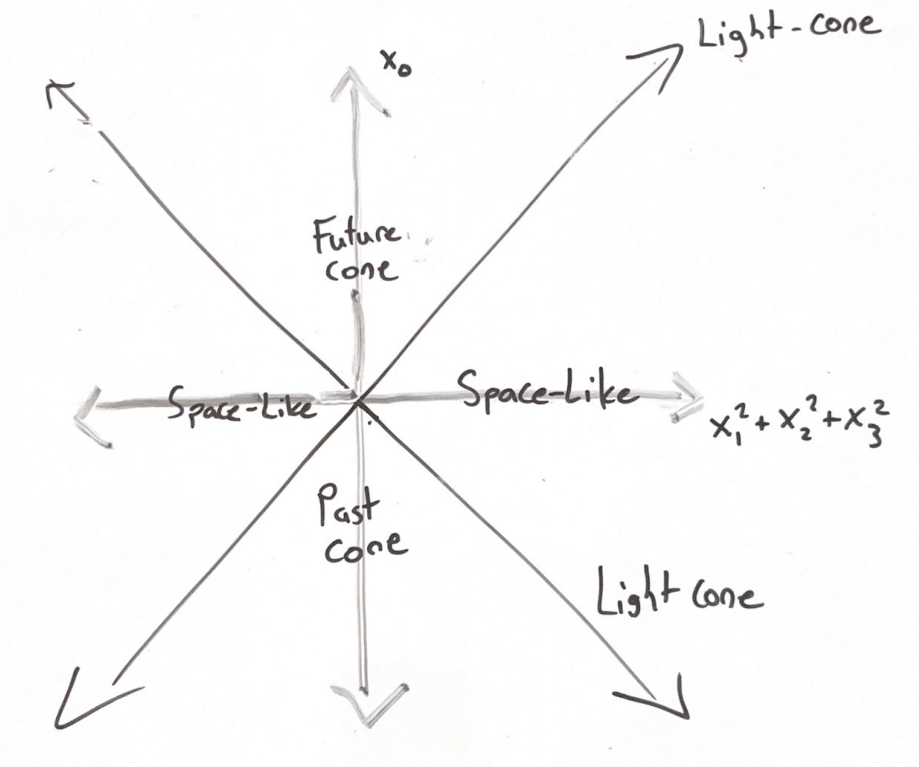
\includegraphics[width=0.7\textwidth]{Light cone-1}
	\caption{Decomposition of Minkowski Space based on length}
\end{figure}

In our study of many other groups in this thesis, group elements have been shown to have helpful decompositions that will make calculations more efficient. The proper Lorentz group is no exception to this.

\begin{theorem} \cite{Tung}
	Any $\Lambda \in \overset{\sim}{L}_+$ can be uniquely written in the following way:
$$\Lambda = R(\theta,\phi,0)L_z(\xi)R(\alpha,\beta,\gamma)^{-1}$$
where $L_z(\xi)$ is a Lorentz boost along the $z$-axis by angle $\xi$ and the parameters for the Euler angles of the rotations from $SO(3)$ are defined as expected.
\end{theorem}

For the sake of clarity, the proof is omitted, as it does not give insight into why this decomposition is possible. One can find more details here.\cite{Tung}

While we have covered what could be crudely considered rotations on Minkowski space, it is relatively straightforward to switch gears and now consider the translations on Minkowski space. Fortunately for us, the construction of these types of operations is very straightforward and is mostly omitted for simplicity. We define the translation group $T_4 = \{T_b \mid b\in\R^4\}$ in the most natural way. It is inherently abelian and will be used to aid us in defining a new group.

\begin{definition}
	The set of all compositions of translations proper Lorentz transformations is called the \textbf{Poincar\'e Group}, denoted $\overset{\sim}{P}$
\end{definition}

Generically speaking, for any transformation in $\overset{\sim}{P}$, any $x\in M$ is mapped into $x'$ in the following way:

\begin{equation}
\begin{aligned}
	x' = \Lambda x + b \text{ for some }\Lambda\in\overset{\sim}{L}_+ \text{ and } b\in\R^4
\end{aligned}
\end{equation}

Much like the Euclidean Group, the composition of any two $g(\Lambda,b),g(\Lambda',b')\in\overset{\sim}{P} $  can be seen to follow the equation below:

\begin{equation}
\begin{aligned}
g(\Lambda,b)g(\Lambda',b') = g(\Lambda\Lambda', \Lambda b' + b)
\end{aligned}
\end{equation}

It is easy to verify that we can embed any $g(\Lambda,b)$ into an invertible $5\times 5$ matrix that acts as the transformation defined by it (embedding four-vectors into a five dimensions space with a trivial component).

$$\begin{bmatrix}
	\underset{4\times 4}{\Lambda} & \underset{4\times 1}{b}\\
	\underset{1\times 4}{0} & \underset{1\times 1}{1}
\end{bmatrix}$$

It can also be easily verified that for any $g(\Lambda,b)\in\overset{\sim}{P}$, there is a natural decomposition of the transformation into:

\begin{equation}
\begin{aligned}
g(\Lambda,b)=T_b\Lambda
 \end{aligned}
\end{equation}


\noindent taking $T_b \sim g(I_4,b)$ and $\Lambda \sim g(\Lambda,0)$.

We can use this identity in a similar manner we did in the Euclidean Group to show that for any $T_b,\Lambda\in\overset{\sim}{P}$, we have

\begin{equation}
\begin{aligned}
	\Lambda T_b \Lambda^{-1} = T_{\Lambda b}
\end{aligned}
\end{equation}

\section{Irreducible Representations of The Poincar\'e Group}

Let us now establish our generators and the Lie Algebra associated with them.

We denote our translational generators $P_\mu$ where $\mu\in\{t,x,y,z\}$. These are defined using identical methodology to the construction of translational generators in $E_2$ and $E_3$. Explicitly, we can write 

\begin{center}
\begin{tabular}{cc}
	$P_t = \begin{bmatrix}
				0 & 0 & 0 & 0 & i \\
				0 & 0 & 0 & 0 & 0\\
				0 & 0 & 0 & 0 & 0\\
				0 & 0 & 0 & 0 & 0\\
				0 & 0 & 0 & 0 & 0\\
			\end{bmatrix}$ &
	$P_x = \begin{bmatrix}
				0 & 0 & 0 & 0 & 0 \\
				0 & 0 & 0 & 0 & i\\
				0 & 0 & 0 & 0 & 0\\
				0 & 0 & 0 & 0 & 0\\
				0 & 0 & 0 & 0 & 0\\
			\end{bmatrix}$ \\
	$P_y = \begin{bmatrix}
				0 & 0 & 0 & 0 & 0 \\
				0 & 0 & 0 & 0 & 0\\
				0 & 0 & 0 & 0 & i\\
				0 & 0 & 0 & 0 & 0\\
				0 & 0 & 0 & 0 & 0\\
			\end{bmatrix}$ &
	$P_z = \begin{bmatrix}
				0 & 0 & 0 & 0 & 0 \\
				0 & 0 & 0 & 0 & 0\\
				0 & 0 & 0 & 0 & 0\\
				0 & 0 & 0 & 0 & i\\
				0 & 0 & 0 & 0 & 0\\
			\end{bmatrix}$
\end{tabular}
\end{center}

and given this, we write any pure translation in $\overset{\sim}{P}$ as 

\begin{equation}
\begin{aligned}
	T_b = e^{-ib_1P_t}e^{-ib_2P_x}e^{-ib_3P_y}e^{-ib_4P_z}
\end{aligned}
\end{equation}

It can then be easily verified with matrix algebra that for any Lorentz transformation (embedded in $M_5(\R)$) the translational generators exhibit the following behavior:

\begin{equation}
\begin{aligned}
	\Lambda P_t \Lambda^{-1} = [\Lambda]_{00}P_t + [\Lambda]_{10}P_x + [\Lambda]_{20}P_y + [\Lambda]_{30}P_z
\end{aligned}
\end{equation}
\begin{equation}
\begin{aligned}
	\Lambda P_x \Lambda^{-1} = [\Lambda]_{01}P_t + [\Lambda]_{11}P_x + [\Lambda]_{21}P_y + [\Lambda]_{31}P_z
\end{aligned}
\end{equation}
\begin{equation}
\begin{aligned}
	\Lambda P_y \Lambda^{-1} = [\Lambda]_{02}P_t + [\Lambda]_{12}P_x + [\Lambda]_{22}P_y + [\Lambda]_{32}P_z
\end{aligned}
\end{equation}
\begin{equation}
\begin{aligned}
	\Lambda P_z \Lambda^{-1} = [\Lambda]_{03}P_t + [\Lambda]_{13}P_x + [\Lambda]_{23}P_y + [\Lambda]_{33}P_z
\end{aligned}
\end{equation}

This should feel like a familiar relationship as we derived in the Euclidean Group (and would likely be the case if we had discussed $E_4$). However, this should allude to the fact that the translational subgroup is intuitively invariant under rotations, and will later be used to search for our invariant subspace. 

We now shift our focus to our generators for rotations. For now, we will consider pure spatial rotations separately from rotations involving a time component. In this sense, we can keep our naming convention by denoting the rotational generator $J_\mu$ where $\mu\in\{x,y,z\}$ to be the rotation about the $\mu$ axis in $\R^3$. Through our similar derivation in $SO(3)$, we recover the following matrices for our generators:


\begin{center}
\begin{tabular}{ccc}
	$J_x = \begin{bmatrix}
				0 & 0 & 0 & 0 & 0 \\
				0 & 0 & 0 & 0 & 0\\
				0 & 0 & 0 & -i & 0\\
				0 & 0 & i & 0 & 0\\
				0 & 0 & 0 & 0 & 0\\
			\end{bmatrix}$ &
	$J_y = \begin{bmatrix}
				0 & 0 & 0 & 0 & 0 \\
				0 & 0 & 0 & i & 0\\
				0 & 0 & 0 & 0 & 0\\
				0 & -i & 0 & 0 & 0\\
				0 & 0 & 0 & 0 & 0\\
			\end{bmatrix}$ &
	$J_z = \begin{bmatrix}
				0 & 0 & 0 & 0 & 0 \\
				0 & 0 & -i & 0 & 0\\
				0 & i & 0 & 0 & 0\\
				0 & 0 & 0 & 0 & 0\\
				0 & 0 & 0 & 0 & 0\\
			\end{bmatrix}$ 
\end{tabular}
\end{center}

Handling the generators of the Lorentz boosts ultimately takes the same form as we have already established. Using the arbitrarily small angle of rotation to create two different ways of computing a generic element, we uncover the following form for our generators of Lorentz boosts: Let $K_m$ where $m\in\{x,y,z\}$ denote the generator of the Lorentz boost along the $m$ axis. Then,

\begin{center}
\begin{tabular}{ccc}
	$K_x = \begin{bmatrix}
				0 & i & 0 & 0 & 0 \\
				i & 0 & 0 & 0 & 0\\
				0 & 0 & 0 & 0 & 0\\
				0 & 0 & 0 & 0 & 0\\
				0 & 0 & 0 & 0 & 0\\
			\end{bmatrix}$ &
	$K_y = \begin{bmatrix}
				0 & 0 & i & 0 & 0 \\
				0 & 0 & 0 & 0 & 0\\
				i & 0 & 0 & 0 & 0\\
				0 & 0 & 0 & 0 & 0\\
				0 & 0 & 0 & 0 & 0\\
			\end{bmatrix}$ &
	$K_z = \begin{bmatrix}
				0 & 0 & 0 & i & 0 \\
				0 & 0 & 0 & 0 & 0\\
				0 & 0 & 0 & 0 & 0\\
				i & 0 & 0 & 0 & 0\\
				0 & 0 & 0 & 0 & 0\\
			\end{bmatrix}$ 
\end{tabular}
\end{center}

As would be expected, any Lorentz transformation can be written in terms of the generators in the following way:

\begin{equation}
\begin{aligned}
	\Lambda (\omega) = e^{-i\omega_1J_x}e^{-i\omega_2J_y}e^{-i\omega_3J_x}e^{-i\omega_4K_x}e^{-i\omega_5K_y}e^{-i\omega_6K_z}
\end{aligned}
\end{equation}

\noindent where $\omega$ is a six-component vector containing values appropriately assigned that decompose $\Lambda$ into rotations in the specified planes. This decomposition can be arrived at with more work using Theorem (5.7). 

At this stage, we can construct a generic element of our Lie algebra, $\mathfrak{\overset{\sim}{p}}$ in the following way. If $A\in\mathfrak{\overset{\sim}{p}}$, 

\begin{equation}
\begin{aligned}A=i
	\begin{bmatrix}
		0 & a & b & c & d\\
		a & 0 & -h & j & e\\
		b & h & 0 & -k & f\\
		c & -j & k & 0 & g\\
		0 & 0 & 0 & 0 & 0\\
	\end{bmatrix}
\end{aligned}
\end{equation}

We can now establish the following commutator relationships through matrix algebra

\begin{equation}
\begin{aligned}
	[P_\mu,P_\nu] = 0 \hspace{3mm} \forall \mu,\nu\in\{t,x,y,z\}
\end{aligned}
\end{equation}
\begin{equation}
\begin{aligned}
	[P_t,P_\mu] = 0 \hspace{3mm} \forall \mu\in\{x,y,z\}
\end{aligned}
\end{equation}
\begin{equation}
\begin{aligned}
	[P_\mu,J_\nu] = \begin{cases}
							0 &\text{if } \mu=\nu \\
							isign(\mu,\nu,\tau)P_\tau & \text{else}
						\end{cases} \hspace{3mm} \forall \mu,\nu,\tau\in\{x,y,z\}\text{ where }\tau \neq\mu,\nu
\end{aligned}
\end{equation}
\begin{equation}
\begin{aligned}
	[P_\mu,K_\nu] = \begin{cases}
							0 &\text{if } \mu=\nu \\
							iP_t & \text{else}
						\end{cases} \hspace{3mm} \forall \mu,\nu\in\{x,y,z\}
\end{aligned}
\end{equation}
\begin{equation}
\begin{aligned}
	[P_t,K_\nu] = iP_\nu \hspace{3mm} \forall\nu\in\{x,y,z\}
\end{aligned}
\end{equation}
\begin{equation}
\begin{aligned}
	[J_\mu,J_\nu] = \begin{cases}
							0 &\text{if } \mu=\nu \\
							isign(\mu,\nu,\tau)J_\tau & \text{else}
						\end{cases} \hspace{3mm} \forall \mu,\nu,\tau\in\{x,y,z\}\text{ where }\tau \neq\mu,\nu
\end{aligned}
\end{equation}
\begin{equation}
\begin{aligned}
	[K_\mu,J_\nu] = \begin{cases}
							0 &\text{if } \mu=\nu \\
							isign(\mu,\nu,\tau)K_\tau & \text{else}
						\end{cases} \hspace{3mm} \forall \mu,\nu,\tau\in\{x,y,z\}\text{ where }\tau \neq\mu,\nu
\end{aligned}
\end{equation}
\begin{equation}
\begin{aligned}
	[K_\mu,K_\nu] = \begin{cases}
							0 &\text{if } \mu=\nu \\
							-isign(\mu,\nu,\tau)J_\tau & \text{else}
						\end{cases} \hspace{3mm} \forall \mu,\nu,\tau\in\{x,y,z\}\text{ where }\tau \neq\mu,\nu
\end{aligned}
\end{equation}

In order to calculate the unitary, irreducible representations of the Poinecar\'e group, we must utilize the same method we used for calculating such representations of $E_3$. To begin, we identify a natural choice for a normal subgroup to quotient out. The easy choice would be $T_4$. Since all the generators of $T_4$ commute, we can conclude that their eigenvectors through the image of any irreducible representation coincide. We sojourn into the universal enveloping algebra to acquire our Casimir elements. In this case, we start by defining a new yet familiar element:

 
\begin{equation}
\begin{aligned}
	\mathfrak{C}_1 \coloneq \mathfrak{P}_t^2 -  \mathfrak{P}_x^2 -\mathfrak{P}_y^2- \mathfrak{P}_z^2
\end{aligned}
\end{equation}

If we assert that $\psi$ is an irreducible representation of $\overset{\sim}{P}$, then we see we see that any eigenvalue of $\psi_{\mathfrak{C}_1}$ need not be strictly positive. Let us denote this eigenvalue as $\lambda_1$. We make note of the ranges for the $\lambda_1$ and separate our tabulation into three cases. For the sake of this thesis, we will only compute the irreducible unitary representations for one of these cases. The rest require work with a more complicated Casimir element than we are used to.

Our case of focus will be when $\lambda_1 > 0$. This means that the time component must be larger in magnitude than all of the spatial components combined. This corresponds to vectors that are time-like. To this end, we pick our starting vector to be $v_0 \coloneq (\sqrt{\lambda_1},0,0,0)$. Taking our anticipated quotient, we can intuitively see that $\overset{\sim}{P}/T_4 \cong \overset{\sim}{L}_+$. We can also see that the largest possible subgroup of this quotient group that leaves time-like vectors invariant would need to be the subgroup isomorphic to $SO(3)$. Therefore, since our little group is isomorphic to $SO(3)$ we will see that every irreducible, unitary representation of $SO(3)$ gives rise to one in $\overset{\sim}{P}$. We recall that for any half or whole positive integer choice of $s$, then we can construct a basis of the subspace corresponding to the image of the little group under $\psi$ in the following way:

\begin{equation}
\begin{aligned}
	\psi_{\mathfrak{J}^2} (v_0)_m = s(s+1)(v_0)_m
\end{aligned}
\end{equation}
\begin{equation}
\begin{aligned}
	\psi_{\mathfrak{J}_z} (v_0)_m = m(v_0)_m
\end{aligned}
\end{equation}
\begin{equation}
\begin{aligned}
	\psi_{\mathfrak{P}_\mu} (v_0)_m = \begin{cases}
										\sqrt{\lambda_1} & \text{if } \mu=t\\
										0 & \text{else}
										\end{cases}
\end{aligned}
\end{equation}

In order to collect a bigger subspace invariant under $\psi$, we deform our initial vector through a general Lorentz transformation. This is straightforward to compute since we have a nice general decomposition of such transformation as seen in (5.7). However, the right-most component of the decomposition of this transformation leaves our vectors invariant (since it is part of $SO(3)$). For clarity, we define a transformation of the following form:

\begin{equation}
\begin{aligned}
	v_p\coloneq H_p((v_0)_m)= R(\alpha,\beta,0)L_z(\xi)(v_0)_m
\end{aligned}
\end{equation}

where ($\alpha$,$\beta$) are the cylindrical coordinates identifying the three-dimensional components of the four-vector $v_p$. This transformation can be applied to change our reference vector to any other vector in $M$. We can generalize the above analysis on each subspace that arises from the little group corresponding to $p$. We recover the entire space by letting $p$ be arbitrary.

\begin{theorem} Time-like Unitary Irreducible Representations of $\overset{\sim}{P}$
	The subspace generated by the vectors $\{(v_p)_m\}_{p,m}$ is invariant under $\overset{\sim}{P}$. The irreducible, unitary representations of elements of this group are characterized in the following way:
$$\psi_{T_b} (v_p)_m = e^{-ib_0p_0}e^{-ib_1p_1}e^{-ib_2p_2}e^{-ib_3p_3}(v_p)_m$$
$$\psi_\Lambda (v_p)_m = [\phi_s(H(p')\Lambda H(p))]_{m'm} (v_{p'})_{m'}$$
where $p' = \Lambda p$ and $\phi_s$ is the irreducible representation of $SO(3)$ defined by $s$.
\end{theorem}

This can be shown in a very similar manner to the methods used in the Euclidean Groups' calculations. 


